%%%%%%預先準備(不需修改)%%%%%%
\documentclass[12pt]{article}
%%%%%%%%%%%字型與中文設定%%%%%%%%%%%
\usepackage{fontspec}
\usepackage{xeCJK}
\setCJKmainfont[AutoFakeBold=3,AutoFakeSlant=.2]{[PMingLiU.ttf]}
\setCJKmonofont{[PMingLiU.ttf]}
\setCJKsansfont{[PMingLiU.ttf]}
\setmainfont[AutoFakeBold=3,AutoFakeSlant=.2]{[times.ttf]}
\setsansfont[AutoFakeBold=3,AutoFakeSlant=.2]{[times.ttf]}
\setmonofont{[times.ttf]}
\newfontfamily\ming[AutoFakeBold=3,AutoFakeSlant=.2]{[PMingLiU.ttf]}
\newfontfamily\timesnew[AutoFakeBold=3,AutoFakeSlant=.2]{[times.ttf]}
\XeTeXlinebreaklocale "zh" %這兩行一定要加,中文才能自動換行
\XeTeXlinebreakskip = 0pt plus 1pt %這兩行一定要加,中文才能自動換行
\usepackage{newtxtext,newtxmath}

%%%%%%%%%%%邊界設定、文字格式%%%%%%%%%%%
\usepackage[margin=2cm, a4paper]{geometry}
\usepackage{indentfirst} 
\setlength{\parindent}{2em}
\usepackage{setspace}
\renewcommand{\baselinestretch}{1.0}
\setlength{\parskip}{1em}
\usepackage[utf8]{inputenc}
\usepackage{changepage} %adjustwidth

%%%%%%%%%%%頁首頁尾%%%%%%%%%%%
\usepackage{fancyhdr}
\pagestyle{fancy}
\renewcommand\headrulewidth{0pt}
\lhead{}
%小論文篇名的部分放在 main 供修改
\rhead{}
\lfoot{}
\cfoot{\fontsize{10pt}{\baselineskip}\selectfont \thepage}
\rfoot{}

% 定義 \XeTeX 符號:
\def\reflect#1{{\setbox0=\hbox{#1}\rlap{\kern0.5\wd0
  \special{x:gsave}\special{x:scale -1 1}}\box0 \special{x:grestore}}}
\def\XeTeX{\leavevmode
  \setbox0=\hbox{X\lower.5ex\hbox{\kern-.15em\reflect{E}}\kern-.1667em \TeX}%
  \dp0=0pt\ht0=0pt\box0 }
\def\XeLaTeX{\leavevmode
  \setbox0=\hbox{X\lower.5ex\hbox{\kern-.15em\reflect{E}}\kern-.0833em \LaTeX}%
  \dp0=0pt\ht0=0pt\box0 }

%%%%%%%%%%%自定義中文數字%%%%%%%%%%%
\newcommand{\CCNumberA}[1]{\ifcase#1\or{壹}\or{貳}\or{參}\or{肆}\or{伍}\or{陸}\or{柒}\or{捌}\or{玖}\or{拾}
    \or{拾壹}\or{拾貳}\or{拾參}\or{拾肆}\or{拾伍}\or{拾陸}\or{拾柒}\or{拾捌}\or{拾玖}\or{貳拾}
    \or{貳拾壹}\or{貳拾貳}\or{貳拾參}\or{貳拾肆}\or{貳拾伍}\or{貳拾陸}\or{貳拾柒}\or{貳拾捌}\or{貳拾玖}\or{參拾}
    \fi}
\newcommand{\CCNumberB}[1]{\ifcase#1\or{一}\or{二}\or{三}\or{四}\or{五}\or{六}\or{七}\or{八}\or{九}\or{十}
     \or{十一}\or{十二}\or{十三}\or{十四}\or{十五}\or{十六}\or{十七}\or{十八}\or{十九}\or{二十}
     \or{二十一}\or{二十二}\or{二十三}\or{二十四}\or{二十五}\or{二十六}\or{二十七}\or{二十八}\or{二十九}\or{三十}
     \or{三十一}\or{三十二}\or{三十三}\or{三十四}\or{三十五}\or{三十六}\or{三十七}\or{三十八}\or{三十九}\or{四十}
     \or{四十一}\or{四十二}\or{四十三}\or{四十四}\or{四十五}\or{四十六}\or{四十七}\or{四十八}\or{四十九}\or{五十}
     \or{五十一}\or{五十二}\or{五十三}\or{五十四}\or{五十五}\or{五十六}\or{五十七}\or{五十八}\or{五十九}\or{六十}
     \or{六十一}\or{六十二}\or{六十三}\or{六十四}\or{六十五}\or{六十六}\or{六十七}\or{六十八}\or{六十九}\or{七十}   
    \fi}

%%%%%%%%%%%章節階層設定%%%%%%%%%%%
\usepackage{titlesec,titletoc}
\setcounter{secnumdepth}{4} %設定計數器使 paragraph 也有編號

\titleformat{\section}                      % #1.改變 section 的指令 
[hang]                                      % #2.將標號及標題視為同一個段落
{\normalfont}                               % #3.標號標題的字形格式
{\\ \CCNumberA{\arabic{section}}、}         % #4.標號
{0pc}                                       % #5.標號標題間隔
{}                                          % #6.標題前之指令
[]                                          % #7.標題後之指令、選擇性輸入

\titleformat{\subsection}                   % #1.改變 subsection 的指令 
[hang]                                      % #2.將標號及標題視為同一個段落
{\normalfont}                               % #3.標號標題的字形格式
{\\ \CCNumberB{\arabic{subsection}}、}      % #4.標號
{0pc}                                       % #5.標號標題間隔
{}                                          % #6.標題前之指令
[]                                          % #7.標題後之指令、選擇性輸入
   
\titleformat{\subsubsection}                % #1.改變 subsubsection 的指令 
[hang]                                      % #2.將標號及標題視為同一個段落
{\normalfont}                               % #3.標號標題的字形格式
{(\CCNumberB{\arabic{subsubsection}})}  % #4.標號
{0pc}                                       % #5.標號標題間隔
{}                                          % #6.標題前之指令
[]                                          % #7.標題後之指令、選擇性輸入

\titleformat{\paragraph}                    % #1.改變 paragraph 的指令 
[hang]                                      % #2.將標號及標題視為同一個段落
{\normalfont}                               % #3.標號標題的字形格式
{\arabic{paragraph}、}                      % #4.標號
{0pc}                                       % #5.標號標題間隔
{}                                          % #6.標題前之指令
[]                                          % #7.標題後之指令、選擇性輸入

\titlespacing{\section} {0em}{0em}{0em}
\titlespacing{\subsection} {2em}{0em}{0em}
\titlespacing{\subsubsection} {4em}{0em}{0em}
\titlespacing{\paragraph} {6em}{0em}{0em}

%%%%%%%%%%%原文照刊環境中文處理(\begin{verbatim})%%%%%%%%%%%
\makeatletter
\def\verbatim@font{\rmfamily} %如果使用roman字体族,将sffamily改成rmfamily
\makeatother
%%%%%%%%%%%列表%%%%%%%%%%%
\usepackage{enumerate}

%%%%%%%%%%%超連結%%%%%%%%%%%
\usepackage{xurl}
\usepackage[bookmarksopen,pdfstartview=FitH,breaklinks=true,
linkcolor=black,anchorcolor=black,citecolor=black,hidelinks]{hyperref}
\urlstyle{same}
%%%%%%%%%%%圖片%%%%%%%%%%%
\usepackage{graphicx}
\usepackage{caption}
\usepackage{float}
\usepackage{subfigure}

%%%%%%%%%%%翻譯中文%%%%%%%%%%%
\renewcommand{\tablename}{表}
\renewcommand{\figurename}{圖}
\renewcommand{\thefigure}{\CCNumberB{\arabic{figure}}}
%%%%%%%%%%%本模版獨特的 new command%%%%%%%%%%%
%打 LaTeX 打不出來的特殊符號
\newcommand\apo{\textquotesingle}

\newcommand{\coverpage}[6]
{
	\begin{titlepage}
		\begin{center}
			投稿類別:#1\\[7cm]
			篇名:\\
			#2\\[6cm]
			作者:\\
		    \if\relax\detokenize{#3}\relax
            
            \else
            #3 \\
            \fi
		    \if\relax\detokenize{#4}\relax
            
            \else
            #4 \\
            \fi
		    \if\relax\detokenize{#5}\relax
            
            \else
            #5 \\
            \fi
			\vfill
			指導老師:\\
			#6
			\end{center}
	\end{titlepage}
}

%頁首
\newcommand{\centerhead}[1]
{
    \chead{\fontsize{10pt}{\baselineskip}\selectfont #1}
}

\newcommand{\h}[1]{\section{#1}}        %令section=h
\newcommand{\hh}[1]{\subsection{#1}}    %令subsection=hh
\newcommand{\hhh}[1]{\subsubsection{#1}}%令subsubsection=hhh
\newcommand{\hhhh}[1]{\paragraph{#1}}   %令paragraph=hhhh

%段落內容及文字縮排(content & text)
\newcommand{\hhtext}[1]
{
    \if\relax\detokenize{#1}\relax
    
    \else
        \begin{adjustwidth}{2em}{0em}
        \hspace*{21pt}#1
        \end{adjustwidth}
    \fi
}
\newcommand{\subsectiontext}[1]
{
    \if\relax\detokenize{#1}\relax
    
    \else
        \begin{adjustwidth}{2em}{0em}
        \hspace*{21pt}#1
        \end{adjustwidth}
    \fi
}
\newcommand{\hhhtext}[1]
{
    \if\relax\detokenize{#1}\relax
    
    \else
        \begin{adjustwidth}{4em}{0em}
        \hspace*{21pt}#1
        \end{adjustwidth}
    \fi
}
\newcommand{\subsubsectiontext}[1]
{
    \if\relax\detokenize{#1}\relax
    
    \else
        \begin{adjustwidth}{4em}{0em}
        \hspace*{21pt}#1
        \end{adjustwidth}
    \fi
}
\newcommand{\hhhhtext}[1]
{
    \if\relax\detokenize{#1}\relax
    
    \else
        \begin{adjustwidth}{6em}{0em}
        \hspace*{21pt}#1
        \end{adjustwidth}
    \fi
}

%%%%%%%%%%%%%%%Reference%%%%%%%%%%%%%%%%%%%%%
%無特定格式
\newcommand{\nonetype}[1]
{
    #1
}
%書籍類
\newcommand{\zhbook}[4]
{
    #1(#2)。\textbf{#3}。#4。
}
\newcommand{\enbook}[4]
{
    \if\relax\detokenize{#1}\relax
        \textit{#3}. (#2). #4.
    \else
        #1. (#2). \textit{#3}. #4.
    \fi
}
\newcommand{\ezhbook}[4]
{
    #1(#2)。\textbf{#3}。\url{#4}
}
\newcommand{\eenbook}[4]
{
    #1. (#2). \textit{#3}. \url{#4}
}
%期刊論文類
\newcommand{\zhjournal}[7]
{
    \if\relax\detokenize{#5}\relax
        #1(#2)。#3。\textbf{#4,#6},#7。
    \else
         #1(#2)。#3。\textbf{#4,#5}(#6),#7。
    \fi
}
\newcommand{\enjournal}[7]
{
    \if\relax\detokenize{#5}\relax
        #1. (#2). #3. \textit{#4, #6}, #7.
    \else
        #1. (#2). #3. \textit{#4,#5}(#6), #7.
    \fi
}
\newcommand{\ezhjournal}[8]
{
    \if\relax\detokenize{#5}\relax
        #1(#2)。#3。\textbf{#4,#6},#7。\url{#8}
    \else
        #1(#2)。#3。\textbf{#4,#5}(#6),#7。\url{#8}
    \fi
}
\newcommand{\eenjournal}[8]
{
    \if\relax\detokenize{#5}\relax
        #1. (#2). #3. \textit{#4, #6}, #7. \url{#8}
    \else
        #1. (#2). #3. \textit{#4,#5}(#6), #7. \url{#8}
    \fi
}
%文集論文類
\newcommand{\zhanthology}[7]
{
    #1(#2)。#3。#4:\textbf{#5}(#6)。#7。
}
\newcommand{\enanthology}[7]
{
    #1.(#2). #3. #4. \textit{#5}, (#6). #7.
}
%博(碩)士論文
\newcommand{\zhthesis}[5]
{
    #1(#2)。\textbf{#3}。#4:#5。
}
\newcommand{\enthesis}[5]
{
    #1. (#2).\textit{#3}. #4: #5.
}
\newcommand{\ezhthesis}[6]
{
    #1(#2)。\textbf{#3}。#4:#5。\url{#6}
}
\newcommand{\eenthesis}[6]
{
    #1. (#2).\textit{#3}. #4: #5. \url{#6}
}
%報紙文章
\newcommand{\zhnewspaper}[5]
{
    #1(#2)。#3。\textbf{#4},#5。
}
\newcommand{\ennewspaper}[5]
{
    #1. (#2). #3. \textit{#4}, #5.
}
\newcommand{\ezhnewspaper}[5]
{
    #1(#2)。#3。\textbf{#4}。\url{#5}
}
\newcommand{\eennewspaper}[5]
{
    #1. (#2). #3. \textit{#4}. \url{#5}
}
%法規
\newcommand{\law}[2]
{
    #1(#2)。
}
%網路相關資源
\newcommand{\simpleinternet}[4]
{
    #1(#2)。#3。\url{#4}
}
\newcommand{\internet}[4]
{
    #1(#2)。#3。\url{#4}
}
\newcommand{\nodateinternet}[4]
{
    #1(無日期)。#2。#3,取自 \url{#4}
}
\newcommand{\youtube}[4]
{
    #1(#2)。#3[影片]。YouTube。\url{#4}
}
\newcommand{\facebook}[5]
{
    #1(#2)。#3[#4]。Facebook。\url{#5}
}
\newcommand{\blog}[4]
{
    #1(#2)。#3[部落格文章]。\url{#4}
}


%%%%%%%%自訂設置(請填入)%%%%%%%%
\centerhead{Android 碳足跡追蹤器開發} %中上方頁首,請填入小論文主題名稱
\pagenumbering{gobble} %移除頁碼
%%%%%%%%文件內容開始%%%%%%%%%%%%
\begin{document}
\coverpage
    {資訊類} %eg.工程技術類
    {Android 碳足跡追蹤器開發} %填入主題名稱
    %填入作者。若作者只有 1 位 或 2 位,則將 {} 內留白即可
    {01 簡仲研。桃園市立武陵高級中學。二年十五班} %第一作者
    {02 李健宇。桃園市立武陵高級中學。二年十五班} %第二作者
    {03 許鈞奕。桃園市立武陵高級中學。二年十五班} %第三作者
    {} %指導老師
    
\section{前言}
    \subsection{研究動機}
        \hhtext {
        最近看新聞時很難不注意到和全球氣候變遷相關的報導,而在生活中也逐漸感受到氣候變遷帶來的影響,例如以前在四五月多時仍不會高到要開冷氣,但是在今年四五月時已經便已經常感到滿頭大汗,並在教室開冷氣。
        }
        \hhtext{在現代社會中,每個人在不管是消費、移動、或者是使用各類電器用品中,都會產生無形的碳排放,但是產生的碳排放中有許多其實可以藉由改變習慣等方式來減少,而本研究是想藉由利用MIT AppInventor 2簡單、程式容易編寫的特性開發製作一款可以紀錄生活中的碳排放,幫助普通人減少碳排放的手機程式。}
        \hhtext{
        手機程式中預計會有計算供人計算碳足跡並儲存每次計算後的結果,以及輸入數值時手機的時間,依據類別來比較當周以及前一周生活中減少或增加的碳排放量。希望藉由能開發出一個實用的碳足跡計算器。
        }
    \subsection{研究目的}
        \subsubsection{了解製作生活碳足跡紀錄APP需要的功能}
        \subsubsection{了解各類碳足跡來源}
        \subsubsection{研究碳足跡計算方法}
        \subsubsection{製作一個碳排放紀錄App}
        
\section{文獻探討}
    \subsection{生活碳足跡對減緩氣候變遷影響}
    \hhtext{生活中個人碳足跡對於能否使幫助減緩全球氣候變遷,從Ryu Koide et al. (2021) 的論文中可看出經過評估後個人可藉由改變生活習慣,能使其生活碳排放減少許多碳排放。要使人能產生對環境友善的生活習慣可藉由習慣形成的方法進行培養,因為習慣與一個人在生活中的各種表現十分相關,而生活環境中的可以藉由各種動作或藉由各種提示會使人在潛意識中傾向去做特定的動作,進而培養習慣 (David T. Neal et al. 2011),因此開發一個能在適當時間提醒並訂定目標的生活碳足跡紀錄工具可以讓人更容易的改變生活方式,進而減少碳足跡。}
    
    \subsection{生活碳排放及計算方式}
    \hhtext{從行政院環境保護署的資料中我們可以看出,對於生活中各類使用的產品以及搭乘的交通工具種類,各自有不同的單位,但是計算結果都以公斤二氧化碳當量(kgCO$_2$e)為單位,對於生活中使用的產品,在產品製造過程中產生的碳排放為產品在其生命週期中乘上一排放係數即可,而二氧化碳當量代表比較溫室氣體相對於二氧化碳造成輻射之單位(廖弓普 2013)。}
    \subsection{AppInventor 程式資料儲存: TinyDB}
    \hhtext{在用AppInventor編寫的手機程式使用的變數再關閉後便會消失,而TinyDB可讓程式在重新起動後繼續存取之前所寫的資料,TinyDB不是關聯式資料庫,資料庫儲存的每個項目有「標籤」(tag)「名稱」(key)「對應值」(value),只能用名稱(key)取出值。參考文華高中BookStack(2019)。}
\section{研究方法}
    \subsection{研究流程}
    \begin{figure}[H] %H代表強制圖片放在原始碼對應的相關位置,htbp代表由 LaTeX 彈性調整
    \captionsetup{format=hang, singlelinecheck=off}
    \centering %圖片置中
    \vspace{0pt}
    \begin{minipage}[t]{0.8\textwidth}
    \caption{以下是我們碳足跡軟體設計的流程圖}
    \centering %圖片在 minipage 置中\
    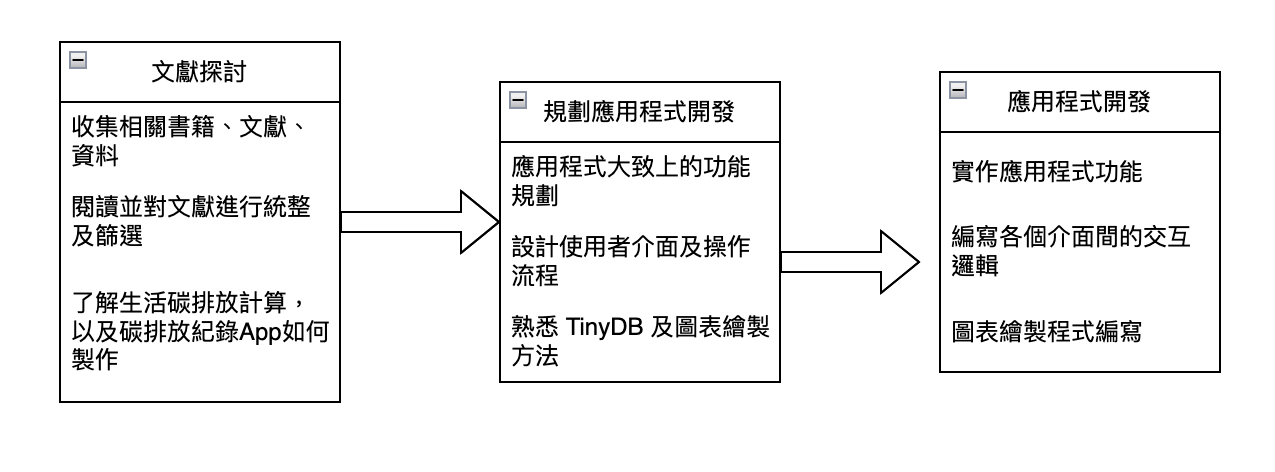
\includegraphics[width=1\textwidth]{研究流程.png}\\[12pt]
    %這裡可以調整相對於 minipage 圖片的比例
    資料來源:作者自行繪製
    \label{fig.flowchart}
    \end{minipage}
    \end{figure}
    
    \subsection{應用程式開發規劃}
    
    \begin{figure}[H] %H代表強制圖片放在原始碼對應的相關位置,htbp代表由 LaTeX 彈性調整
    \captionsetup{format=hang, singlelinecheck=off}
    \centering %圖片置中
    \vspace{0pt}
    \begin{minipage}[t]{0.8\textwidth}
    \caption{以下是我們開發碳足跡軟體的流程圖}
    \centering %圖片在 minipage 置中\
    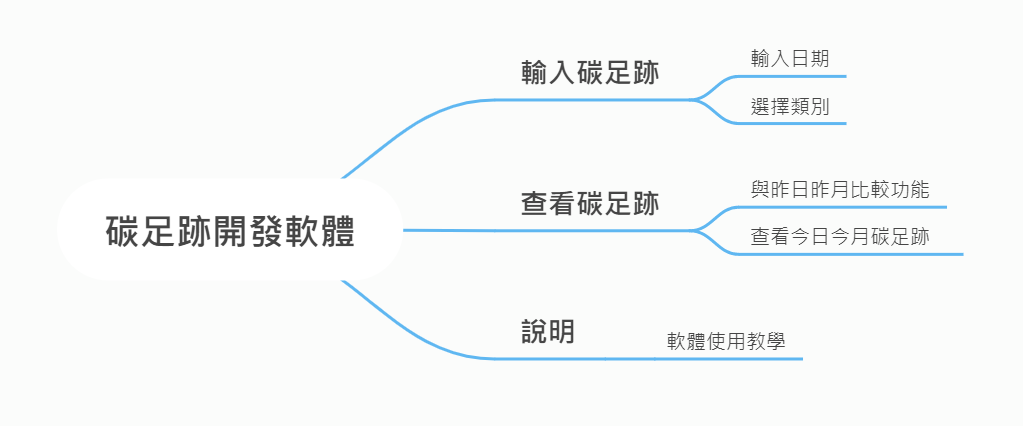
\includegraphics[width=1\textwidth]{流程圖.png}\\[12pt]
    %這裡可以調整相對於 minipage 圖片的比例
    資料來源:作者自行繪製
    \label{fig.plan}
    \end{minipage}
    \end{figure}

    \hhtext{我們編寫的手機程式決定以圖二的架構來編寫,程式包含讓人以進行活動的類別來計算產生的碳排放的功能,除了計算並記錄的功能外程式有一個介面專門用來讓使用者分別檢視以週和月來查看並比較自己過去和現在產生的碳排放。}

    \subsection{應用程式開發}
    \hhtext{我們在設計規劃完應用程式的大致功能後,我們便開始進行程式開發,開發過程共有三大目標}
    \subsubsection{實作應用程式功能}
    \subsubsection{編寫各個應用程式介面間的交互邏輯}
    \subsubsection{碳足跡資料儲存及圖表繪製程式編寫}
    
\section{研究分析與結果}
    \subsection{應用程式概覽}
    \hhtext{我們的手機程式共分成兩大主要功能}
    \subsubsection{登錄並計算碳排放資料}
    \subsubsection{查看碳足跡統計資料}
    \hhtext{剛啟動程式時,首先使用者會看到的是如圖三的應用程式初始介面,在這個介面中使用者有三個選項,分別為:新增碳足跡、查看日碳足跡、查看月碳足跡及應用程式說明。}
    \begin{figure}[H] %H代表強制圖片放在原始碼對應的相關位置,htbp代表由 LaTeX 彈性調整
        \captionsetup{format=hang, singlelinecheck=off}
        \centering %整組合併的圖片置中
        \vspace{0pt}
        \begin{minipage}[t]{0.45\textwidth} %可調整子圖區域大小,但所有 minipage 總合不能超過 1
            \centering %在圖片的 minipage 內置中
            \caption{應用程式初始頁面}
            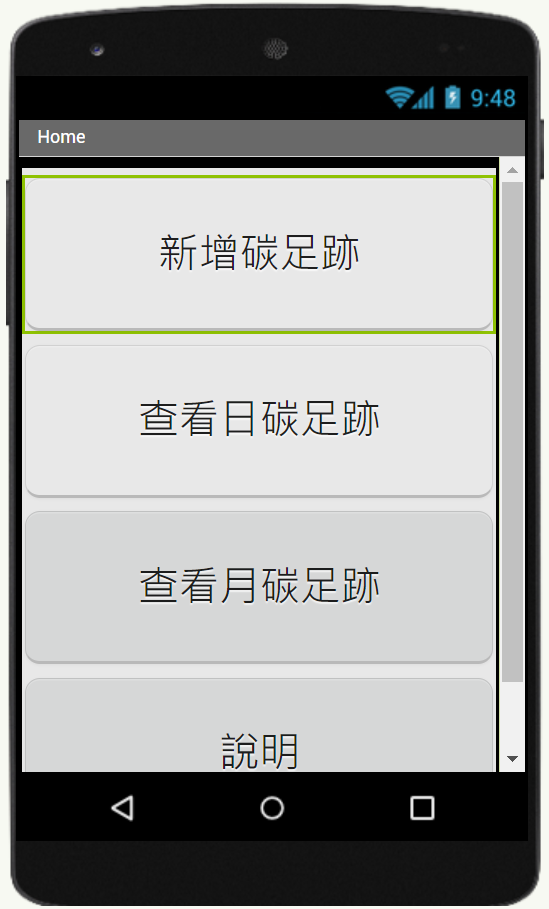
\includegraphics[width=0.7\textwidth]{首頁.png}\\[12pt]
            %圖片相對於 minipage 要多寬
            資料來源:作者自行截圖
            \label{fig.2}
        \end{minipage}
        \begin{minipage}[t]{0.45\textwidth}
            \centering
            \caption{新增碳足跡資料}
            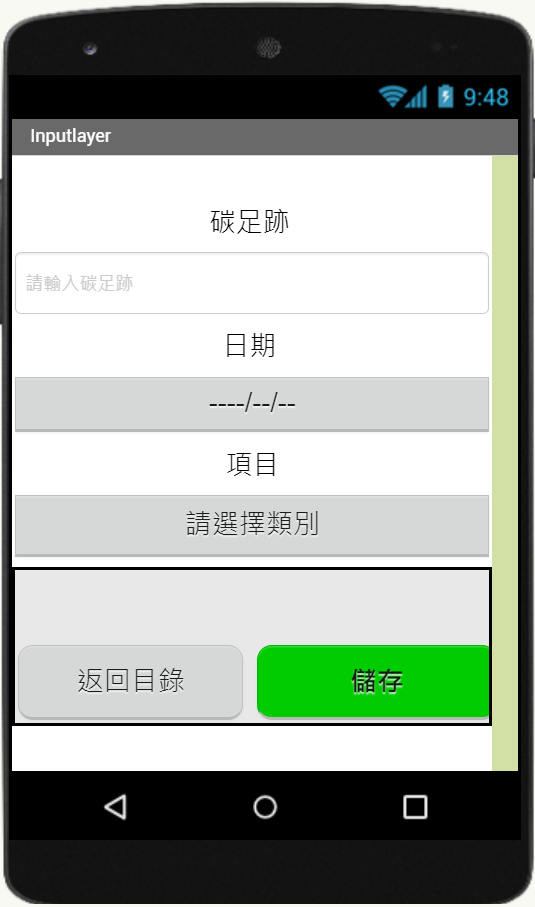
\includegraphics[width=0.7\textwidth]{新增資料.png}\\[12pt]
            資料來源:作者自行截圖
            \label{fig.3}
        \end{minipage}
    \end{figure}
    \hhtext{當使用者要輸入統計資料,便會進入如圖四的碳足跡資料新增介面,在這個介面中,使用者會被要求選擇類別,而根據選擇的類別,上方輸入碳足跡的輸入方塊會根據選擇的類別而改變為相對應的輸入單位提示,在使用者邊輸入時,程式會同時會計算並在儲存按鈕上的灰色框中顯示出以二氧化碳當量CO$_2$e 計算出的輸出單位。}

    \begin{figure}[H] %H代表強制圖片放在原始碼對應的相關位置,htbp代表由 LaTeX 彈性調整
    \captionsetup{format=hang, singlelinecheck=off}
    \centering %圖片置中
    \vspace{0pt}
    \begin{minipage}[t]{0.8\textwidth}
    \caption{每日資料檢視}
    \centering %圖片在 minipage 置中\
    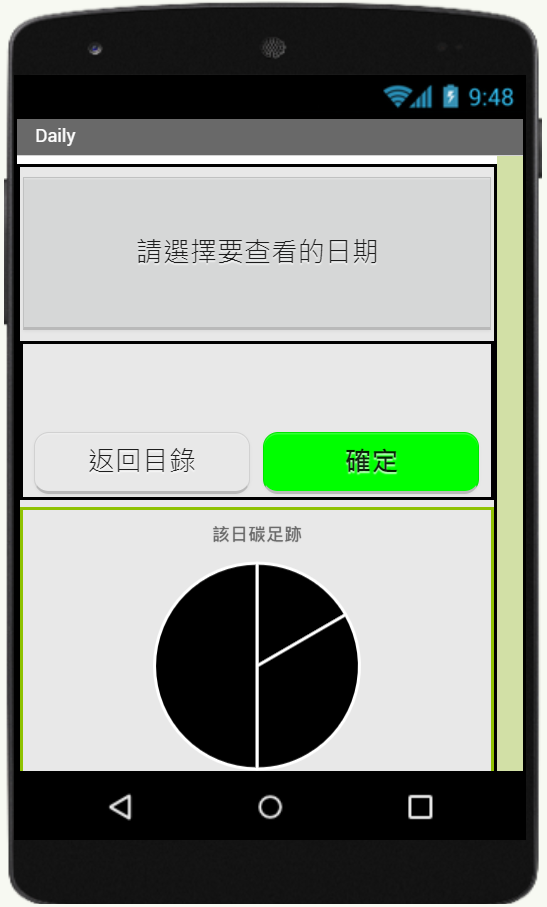
\includegraphics[width=0.45\textwidth]{每日資料檢視.png}\\[12pt]
    %這裡可以調整相對於 minipage 圖片的比例
    資料來源:作者自行截圖
    \label{fig.viewdata}
    \end{minipage}
    \end{figure}
    
    \hhtext{當使用者要檢視以日為單位的碳足跡排放資料時,便會進到如圖五的碳足跡檢視介面,在這個介面中使用者預設會看到一個圓餅圖看出當天各類別的碳足跡占比,在這介面中使用者也可以檢視過去的碳足跡資料。}
    \subsection{程式運作-程式資料處理}
    \begin{figure}[H] %H代表強制圖片放在原始碼對應的相關位置,htbp代表由 LaTeX 彈性調整
    \captionsetup{format=hang, singlelinecheck=off}
    \centering %圖片置中
    \vspace{0pt}
    \begin{minipage}[t]{0.8\textwidth}
    \caption{使用者資料處理程式(部分)}
    \centering %圖片在 minipage 置中\
    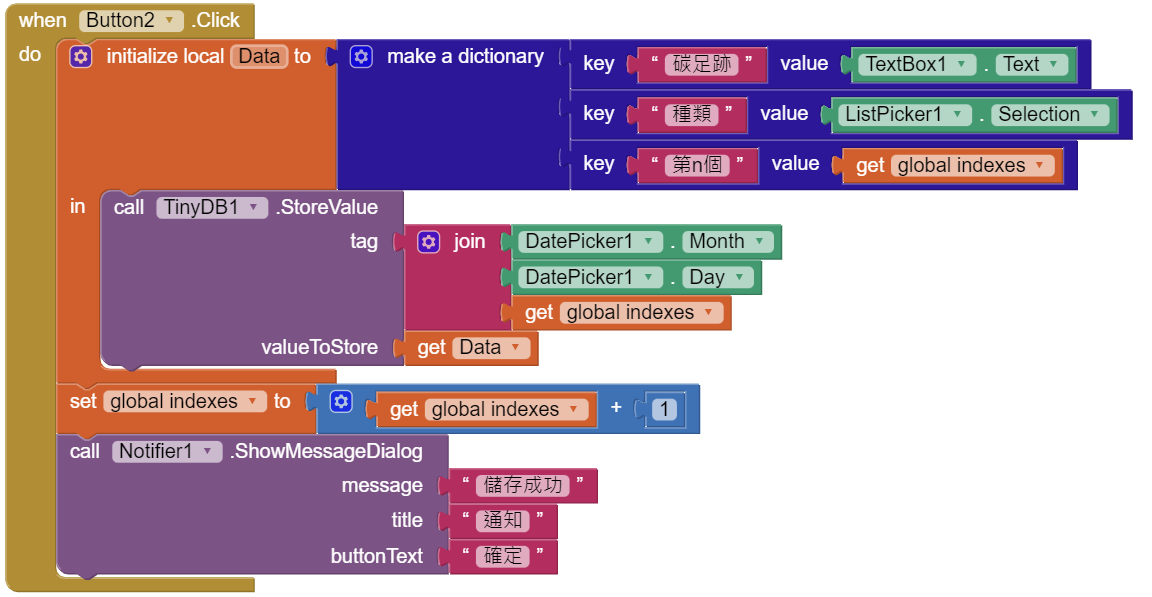
\includegraphics[width=0.7\textwidth]{碳足跡資料儲存程式.png}\\[12pt]
    %這裡可以調整相對於 minipage 圖片的比例
    資料來源:作者自行截圖
    \label{fig.dataprogram}
    \end{minipage}
    \end{figure}
    \hhtext{在處理前面圖三介面的使用者輸入資料時,我們會先將輸入的資料根據相對應的類別乘上計算公式並將計算後的數值放到 Textbox1 也就是儲存按鈕上的灰色框中供使用者檢視,當使用者按下圖三畫面中的儲存資料按鈕後,便會進行圖六的資料處裡程式,程式先會將計算數值、種類、當天第n比做成一個Dictionary方便計算圖表時提取資料,再使用TinyDB元件製作一個TinyDB項目進行資料儲存,我們利用日期作為標籤(tag)、對應值(valueTostore)則用先前製作出來的Dictonary儲存,因此之後在提取資料時需要新建一個空白Dictionary來提取項目中的資料。}

    \subsection{應用程式測試}
    \hhtext{在程式編寫完後,我們有實際安裝應用程式到自己的手機上進行測試,一開始實際使用時覺得功能都運作良好,基本圖表繪製、儲存功能都可正常使用,但是在使用過程中,我們發現這個程式雖然能這正常使用,但是在紀錄碳足跡的功能,我們一致的認為單位輸入有些麻煩,因此使用者輸入的資料會有些簡略,像是要計算搭車產生的碳足跡,需要輸入搭車的距離,使用者在使用時通常不會輸入精確的數據,導致結果和實際差異大,因此會影響應用程式的統計以及比較功能。}
\section{研究結論與建議}
\hhtext{雖然我們成功開發出整個程式,但考慮到碳足跡的計算並無如以上所述容易計算,需要考眾多因素,導致我們輸入的值只是估計的理論值,況且我們也沒有辦法得知其他碳排放行為的碳足跡,使得個人碳足跡排放量無法被全部考量。但是若我們能夠確切的得知所有行為的準確碳排放量或得知使用者的資料庫,程式只要過優化,像是:跟全球平均做比對、提醒使用者哪個方面的碳排放行為可以減少,我們相信還是有可用之處。在市面上我們發現了Klima-Live carbon neutral這款App跟我們的理念幾乎相同,且這款App還會建議使用者可以做出哪些改善來降低碳排放,明顯符合我們的理念。}

\section{參考文獻}

%%%%%%%%%%%%%%%%%%%%%%%%%%%%%%%%%%%%%%%%%%%%%
%此區塊為參考文獻,請直接編輯 ref.tex 檔案%

\begin{enumerate}[(1)]
%%%%%%%%請從 copy[ref].tex 中複製需要的指令來修改%%%%%%
%%%\item \blog
%{侯竣奇}
%{2022年7月6日}
%{LaTeX 小論文模板 README}
%{https://junqi.netlify.app/latexsmallessaytemplate}
%%%

% \item \simpleinternet
% {中學生網站} %網站名稱
% {110 年 2 月 17 日} %登載年月日
% {全國高級中等學校小論文寫作比賽格式說明暨評審要點} %文章名稱
% {https://reurl.cc/Wr2p7D} %網址(可用短網址)

\item \eenjournal
{Ryu Koide, Michael Lettenmeier, Lewis Akenji, Viivi Toivio, Aryanie Amellina, Aditi Khodke, Atsushi Watabe \& Satoshi Kojima } %作者
{2021 August 11} %出版年月日(注意年月日都要)
{Lifestyle carbon footprints and changes in lifestyles to limit global warming to 1.5 C, and ways forward for related research} %文章名稱
{Springer Link Sustainability Science} %期刊名稱
{16} %卷(若無卷/期之分,這格請留白)
{2021}%期(若無卷期之皆則填入卷)
{2087–2099} %頁碼
{ https://link.springer.com/article/10.1007/s11625-021-01018-6 }

\item \eenjournal
{David T. Neal, Wendy Wood, Jennifer S. Labrecque, \&Phillipa Lally} %作者
{2011 July 26} %出版年月日(注意年月日都要)
{How do habits guide behavior? Perceived and actual triggers of habits in daily life} %文章名稱
{Journal of Experimental Social Psychology} %期刊名稱
{48} %卷(若無卷/期之分,這格請留白)
{2}%期(若無卷期之皆則填入卷)
{492-498} %頁碼
{ https://www.sciencedirect.com/science/article/abs/pii/S0959652611004409 }

\item \simpleinternet
{行政院環境保護署}
{112 年 5 月 15 日}
{碳足跡排放係數}
{ https://data.epa.gov.tw/dataset/detail/CFP_P_02 }

\item  \simpleinternet
{廖弓普}
{2013 年 8 月 8 日}
{行政院環境保護署產品與服務碳足跡計算指引}
{https://shorturl.at/qwALR}

\item \simpleinternet
{文華高中BookStack}
{2019 年 5 月 11 日}
{App Inventor 2練習:微型資料庫(TinyDB)}
{ https://shorturl.at/grvyI }


\end{enumerate}
%%%%%%%%%%%%%%%%%%%%%%%%%%%%%%%%%%%%%%%%%%%%%

\end{document}
